\hypertarget{introduction}{%
\section{Introduction}\label{introduction}}

\hypertarget{method}{%
\subsection{Method}\label{method}}

!! Say something to the effect that all data and code are available on
GitHub.

!! In this chapter, the prototype for a machine indexing of Edoc is
presented. The focus is primarily on practical implementation although
care is taken to spell out design decisions in as much detail as is
needed.

\hypertarget{outline}{%
\subsection{Outline}\label{outline}}

Let us start by stating the aim of the prototype. From a functional
perspective, the prototype takes a subset of the data from Edoc as input
and provides index terms for each item in this subset as output. In
order to fulfill this aim we can distinguish a number of steps that need
to be taken:

\begin{enumerate}
\def\labelenumi{\arabic{enumi}.}
\tightlist
\item
  Understand the Edoc data.\\
\item
  Select and construct a sample data set.
\item
  Use Annif to index the items in the sample data set.
\item
  Construct a gold standard from the keywords.
\item
  Assess the quality of the output based on the gold standard.
\end{enumerate}

In the sections below, these steps will be discussed in detail.

\hypertarget{tools}{%
\subsection{Tools}\label{tools}}

For data refinement I use OpenRefine version 3.4.1
(https://openrefine.org/). Data manipulation in OpenRefine is tracked:
the manipulation history of some data can be exported as JSON file and
then reproduced (on the same data on a different machine or on different
data) by loading said file. I will supply a corresponding manipulation
history whenever appropriate. Note that when using OpenRefine with
larger files (and there are many such files in this project), the memory
allocation to OpenRefine must be manually increased (see
https://docs.openrefine.org/manual/installing/\#increasing-memory-allocation
for details). Also note that OpenRefine always counts the number of
records by the first column (a fact which caused me many headaches).

\hypertarget{edoc-data}{%
\section{Edoc data}\label{edoc-data}}

\hypertarget{edoc-and-data-extraction}{%
\subsection{Edoc and data extraction}\label{edoc-and-data-extraction}}

Edoc is the institutional repository of the University of Basel. It was
conceived in 2009 as repository for electronic dissertations and grew in
scope when the University of Basel adapted its first open access policy
in 2013. As per today Edoc contains roughly 68'000 items. Edoc runs on
the EPrints 3 document management system
(https://github.com/eprints/eprints).

Even though Edoc is a public server, its database does not have a
web-ready API. In addition, since Edoc is a production server, its
underlying database cannot be used directly on pain of disturbing the
provided services. The data hence needs to be extracted from Edoc in
order to work with it. This could for example be achieved by cloning the
database of the server and running it on a local machine. However, this
route was not available due to the limited resources of the responsible
co-workers. I thus employed a workaround: Edoc has a built-in advanced
search tool where the results can be exported. Even though it is not
possible to extract all database items by default, only one of the many
available search fields has to be filled in. The complete database can
hence be extracted by only filling in the \texttt{Date} field and using
a sufficiently permissive time period such as 1940 to 2020 since the
oldest record in the database was published in 1942. On January 21 2021,
this query yielded 68'345 results. These results were then exported as a
326 MB JSON file called \texttt{1942-2020.json}. \texttt{1942-2020.json}
has two drawbacks. First, the maximum file size on GitHub is 100 MB. And
second, \texttt{1942-2020.json} is too big to be handled by standard
editors requiring special editors such as Oxygen. For these reasons
\texttt{1942-2020.json} was split into smaller files that are easier
handled and can be uploaded to GitHub. For this
\texttt{Utility.split\_json} was used yielding 14 files of size 20 MB or
less containing 5000 or fewer entries each. These files are called
\texttt{raw\_master\_x-y.json} (where x and y indicate the entries as
given by \texttt{1942-2020.json}) and saved under \texttt{/edoc/raw}.

\hypertarget{data-description-and-analysis}{%
\subsection{Data description and
analysis}\label{data-description-and-analysis}}

!! Explain the Edoc data fields. Say perhaps something about the
granularity of the relevant fields. Say something about how the fields
are filled in (and by whom).

\hypertarget{sample-data-set}{%
\section{Sample data set}\label{sample-data-set}}

In this section, I will explain how the sample data set is selected and
constructed. ``Selection'' means the task of specifying a subset of the
Edoc data and ``construction'' means the task of implementing this
selection.

\hypertarget{selection}{%
\subsection{Selection}\label{selection}}

There are a number of constraints for selecting the sample data set
pertaining to an items's text, evaluability and the data set's scope.

The first constraint stems from Annif, the machine indexing framework
that will be used. Put simply, machine indexing assigns index terms to a
text based on training data. The training data consists of a set of
texts, a vocabulary, and function from vocabulary to texts. In this
context we mean by ``text'' a sequence of words in a natural language
and by ``vocabulary'' a set of words. Intuitively, the training data
consists of pairs of text and subject terms that meet some standard. The
training data and the vocabulary are already supplied by Annif, we only
need to provide a text for each item that we want to be assigned index
terms. Therefore, we only select items with text.

The second constraint is that we must be able to evaluate the quality of
the index terms assigned by Annif to any item in the sample data set.

The third and final constraint takes into account the possibility of
having to extend the prototype to the complete Edoc data. On the one
hand, the sample data set should be small enough to allow for easy
handling and rapid iteration. On the other hand, the sample data set
should not be trivial but reflect the quirks and inadequacies of the
complete dataset. In other words, we are looking for an abstraction
rather than an idealization in the sense of Stokhof and van Lambalgen
(2011).

\hypertarget{construction}{%
\subsection{Construction}\label{construction}}

The first constraint is that each item in the sample data set needs to
have a text. Intuitively, this text could consist of a title, an
abstract, or even a full text, or any combination of the above. Similar
to manual indexing, having more information (that is, longer texts)
usually implies a higher indexing quality in machine indexing. However,
this assumption needs to be confirmed empirically for the given machine
indexing framework and data set. If indeed confirmed, it might be
advisable only to index items that have a certain minimal text length.
Therefore, in order to construct the sample data set, we require each
item to have a non-empty value in the data fields \texttt{title},
\texttt{abstract}, and \texttt{id\_number} as proxy to retrieve a full
text remotely. Note that even more context could be provided by taking
into account other data fields such as \texttt{type},
\texttt{publication} or \texttt{department}. Especially the latter might
be valuable when disambiguating homonymous or polysemous words. For
example, consider the item
\texttt{https://edoc.unibas.ch/id/eprint/76510} which is titled
``Blacking Out.'' Without further context, this title could refer
(amongst others) to a physiological phenomenon, a sudden loss of
electricity, or a measure taken in wartime. Knowing that the item was
published by a researcher employed by the Faculty of Business and
Economics (and not, say, by the Faculty of Medicine) gives us reason to
exclude the first meaning. However, this idea cannot be implemented with
the out of the box instance of Annif employed in this chapter (see
\protect\hyperlink{machine-indexing}{subsection ``Machine indexing''}).

The second constraint is that the index terms assigned to each item in
the sample data set must be assessable. How the assessment is conducted
in detail is discussed in \protect\hyperlink{assessment}{section
``Assessment''}. For now, it is sufficient to say that we require a
standard against which we can evaluate the assigned index terms. By
``standard'' I mean that given a vocabulary of index terms and our
sample data set, for every item in the sample data set, there is an
approved subset of the vocabulary. The production of a standard from
scratch is of course is very costly since a person, usually highly
skilled in a certain academic domain, must assign and/or approve each
item's index terms (!!source). For this reason we try to avoid having to
produce a standard. One way of doing so is by requiring items in the
sample data set to have non-empty \texttt{keywords} data field. The
caveats of this approach are discussed in
\protect\hyperlink{assessment}{section ``Assessment''}.

Taking into account the third constraint simply means that we do not
employ any further restrictions. We can hence construct the sample data
set by choosing exactly those items from \texttt{/edoc/raw} which have
non-empty data fields \texttt{title}, \texttt{abstract},
\texttt{id\_number}, and \texttt{keywords}. We do so by calling
\texttt{Data.select\_from\_file} iteratively for all files in
\texttt{/edoc/raw}. The resulting file is saved in
\texttt{/edoc/selected} as \texttt{selected\_master.json}.

\hypertarget{analysis}{%
\subsection{Analysis}\label{analysis}}

Of the 68'345 items in \texttt{/edoc/raw}, all have a title (non-empty
\texttt{title} data field), a little more than half of the items have an
abstract (37'381 items with non-empty \texttt{abstract} data field),
roughly half of the items have an ID (35'355 items with non-empty
\texttt{id\_number} data field),\footnote{Note that when using the facet
  by blank on \texttt{id\_number} in OpenRefine, there are 57'153
  matches; this is due to the fact that many items with an ID such as
  DOI have secondary or tertiary IDs such as ISI or PMID.} and less than
10\% of the items have keywords (6'660 items with non-empty
\texttt{keywords} data field). The sample data set as requires all the
above data fields to be non-empty;
\texttt{/edoc/sample/sample\_master.json} has 4'111 items and hence
constitutes 6\% of the raw data.

In order to determine how well the sample data set represents the raw
Edoc data, a one-sample \(\chi^2\) goodnes of fit test was conducted on
each selection data field (following Parke 2013, chap. 1). The results
indicate that the sample data proportions of items are significantly
different from the raw Edoc data per department (see Figure 1 for more
details).

\begin{figure}
\centering
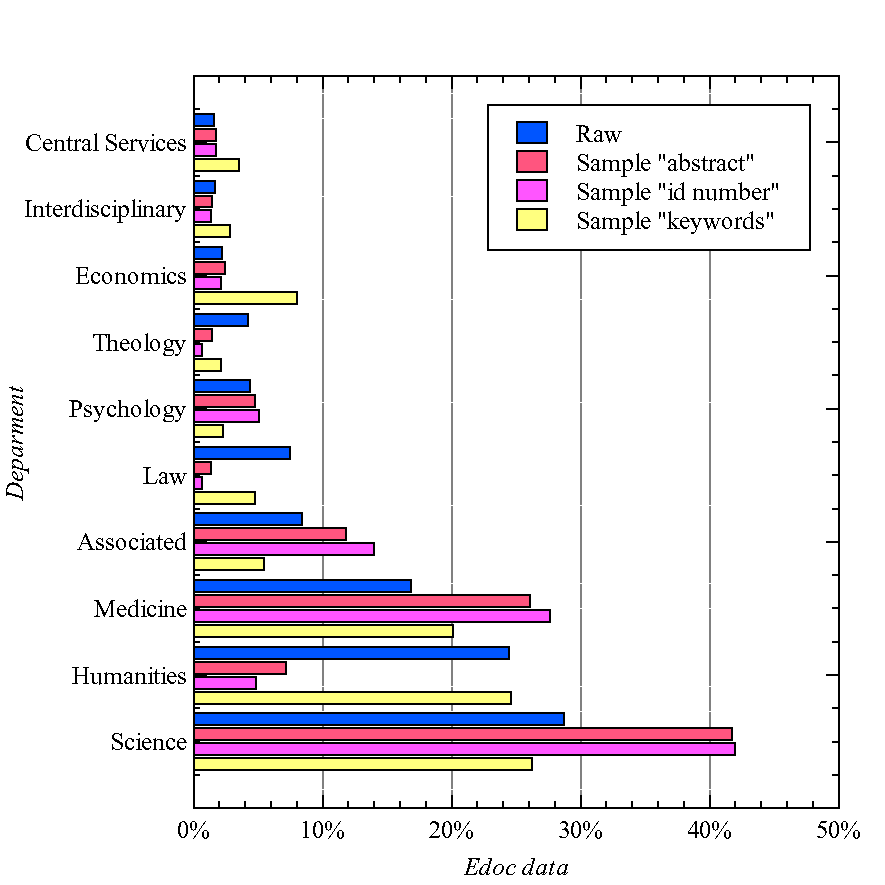
\includegraphics{images/chi_square_selection_fields.pdf}
\caption{The sample data set (\(n\) = 4'111) is not representative of
the raw Edoc data per department. Data field \texttt{abstract}:
\(\chi^2 (df=9) =\) 3'160.556, \(p < 0.001\); data field
\texttt{id\_number}: \(\chi^2 (df=9) =\) 4'209.0285, \(p < 0.001\); data
field \texttt{keywords}: \(\chi^2 (df=9) =\) 2'314.533, \(p < 0.001\).
The data foundation is available at
\texttt{/edoc/analysis/chi\_square\_\{data\ field\}} and the
\(\chi^2\)-statistic can be calculated by calling
\texttt{Analysis.print\_chi\_square\_fit} on the data foundation files.}
\end{figure}

The sample data set is hence not representative of the raw Edoc data.
This is not surprising since its construction is strongly biased. This
bias has the effect that the sample data set is significantly skewed
towards English journal publications in the sciences, medicine and
economics from the 21st century (again, this is shown by a one-sample
\(\chi^2\) goodness of fit test, see Figure 2 for more details). The
upshot of this analysis is that the humanities are underrepresented in
the sample data set. Therefore, any results with respect to the quality
of machine indexing discussed below might not be applicable to the
humanities.

\begin{figure}
\centering
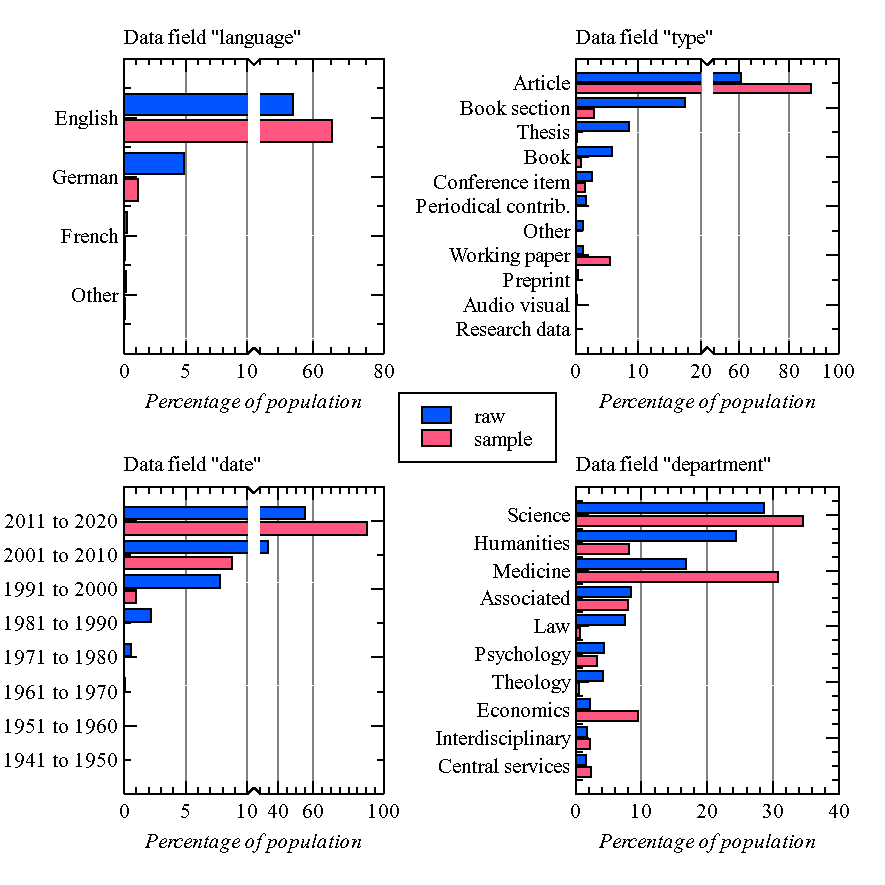
\includegraphics{images/raw_sample_analysis.pdf}
\caption{The sample data set (\(n\) = 4'111) is significantly skewed
towards English (data field \texttt{language}: \(\chi^2 (df=3) =\)
1'441.414, \(p < 0.001\)) journal publications (data field
\texttt{type}: \(\chi^2 (df=10) =\) 52'519.743, \(p < 0.001\)) in the
sciences, medicine and economics (data field \texttt{department}:
\(\chi^2 (df=9) =\) 14'447.276, \(p < 0.001\)) from the 21st century
(data field \texttt{date}: \(\chi^2 (df=7) =\) 35'878.493,
\(p < 0.001\)) as compared to the raw Edoc data. The data foundation is
available at \texttt{/edoc/analysis/chi\_square\_\{data\ field\}} and
the \(\chi^2\)-statistic can be calculated by calling
\texttt{Analysis.print\_chi\_square\_fit} on the data foundation files.}
\end{figure}

\hypertarget{machine-indexing}{%
\section{Machine indexing}\label{machine-indexing}}

\hypertarget{general-overview}{%
\subsection{General overview}\label{general-overview}}

!! Give an overview over machine indexing.

\hypertarget{annif}{%
\subsection{Annif}\label{annif}}

!! Given an intro to Annif. Explain that we are using the out of the box
version

\hypertarget{implementation}{%
\subsection{Implementation}\label{implementation}}

As explained above, for the prototype we will use the out

!! Explain how to implementation works.

In addition to the already used algorithms we should also try
https://ai.finto.fi/?locale=en

!! Somewhere here we talk about indexing based on title and/or abstract
and/or fulltext. Fulltext is not yet implemented. Some observations to
do so: - the link to the fulltext is constructed from the data fields
\texttt{offical\ url} and \texttt{documebts\ -\ main}, e.g.,
\texttt{https\ \ ://edoc.unibas.ch/79633/} + \texttt{1/} +
\texttt{2020\_18\_Informed\ by\ wet\ feet\_How\ do\ floods\ affect\ property\ prices.pdf}
to get
\texttt{https://edoc.unibas.ch/79633/1/2020\_18\_Informed\ by\ wet\ feet\_How\ do\ floods\ affect\ property\ prices.pdf}

\hypertarget{gold-standard}{%
\section{Gold standard}\label{gold-standard}}

In this section I will construct a derivative gold standard in order to
assess the quality of machine indexing the sample data set with Annif.

\hypertarget{definition}{%
\subsection{Definition}\label{definition}}

The most common approach for assessing the output of machine indexing is
by systematically comparing it with a gold standard (sometimes also
referred to as model or reference). Golub et al. (2016, 10) define a
gold standard as ``a collection in which each document is assigned a set
of {[}subject terms{]} that is assumed to be complete and correct''
where ``\emph{complete} means that all subjects that should be assigned
to a document are in fact assigned, and \emph{correct} means that there
are no subjects assigned that are irrelevant to the content.'' Put
inversely, if an item in the gold standard lacks subject terms
describing its content, the assignment is not complete; and if an item
in the gold standard has been assigned subject terms that are not
relevant to its content, the assignment is not correct.

A gold standard is usually the product of manual indexing by
``information experts, subject experts, or potential or real end users''
(Golub et al. 2016, 10). This entails its own host of epistemic problems
relating to objectivity and consistency of the assigned subject terms.
Most importantly, however, the construction of a gold standard from
scratch is very expensive. It is therefore not an option for the project
at hand. Rather, I will construct what could be called a ``derivative''
gold standard by reusing indexing data that is already available.

There are other methods for assessing machine indexing quality besides
comparison with a gold standard that are worth mentioning. These include
an evaluation in the context of indexing workflows (Golub et al. 2016,
13ff.), the assessment of retrieval performance (Golub et al. 2016,
15--23.), and so-called model free assessments (Louis and Nenkova 2013).

The construction of the derivative gold standard takes x steps:

\begin{enumerate}
\def\labelenumi{\arabic{enumi}.}
\tightlist
\item
  Extract the keywords from the sample data set.\\
\item
  Clean the extracted keywords.
\item
  Reconcile the extracted keywords with\ldots{}
\end{enumerate}

The intended output of this transformation process is\ldots{}

These steps are explained in more detail in what follows.

\hypertarget{extract-and-clean-keywords}{%
\subsection{Extract and clean
keywords}\label{extract-and-clean-keywords}}

In a first step, the keywords must be extracted from the sample data set
\texttt{/sample/sample\_master.json}. Recall that we mandated a
non-empty \texttt{keywords} data field for an item to be selected from
the raw Edoc data (see \protect\hyperlink{selection}{subsection
``Selection''}). We can thus simply copy the information in the
\texttt{keywords} data field on a per item basis. To do this, we call
\texttt{Keywords.extract\_keywords} with the sample data set as argument
and save the output as \texttt{keywords/keywords\_extracted.json} like
so:

\begin{Shaded}
\begin{Highlighting}[]
\NormalTok{keywords }\OperatorTok{=}\NormalTok{ Keywords.extract\_keywords(DIR }\OperatorTok{+} \StringTok{"/sample/sample\_master.json"}\NormalTok{)}
\NormalTok{Utility.save\_json(keywords, DIR }\OperatorTok{+} \StringTok{"/keywords/keywords\_extracted.json"}\NormalTok{)}
\end{Highlighting}
\end{Shaded}

In second step, a list of all single keywords must be created. In order
to do so, let us consider now in more detail the exact information
extracted from the \texttt{keywords} data fields as per
\texttt{/keywords/keywords\_extracted.json}. In Edoc, the
\texttt{keywords} data field of an item is a non-mandatory free text
field that is filled in by the user (usually one of the authors) who
undertakes the data entry of an item to Edoc. Even though the Edoc user
manual specifies that keywords must be separated by commas (Universität
Basel, n.d., 8), this requirement is neither validated by the input mask
nor by an administrator of Edoc. Furthermore, neither the manual nor the
input mask provide a definition of the term ``keyword.'' A vocabulary or
a list of vocabularies from which to choose the keywords is also
lacking. Taken together, these observations are indicative of very
heterogeneous data in the \texttt{keywords} data field. To wit, the
items of \texttt{/keywords/keywords\_extracted.json} are strings where
single keywords are individuated by any symbols the user saw fit. So,
for each item in \texttt{/keywords/keywords\_extracted.json}, the user
input must be parsed into single keywords.

Next the so parsed single keywords must be cleaned or normalized: we
want the keywords to follow a uniform format thereby joining
morphological duplicates such as ``Gene,'' ``gene,'' ``gene\_,''
``gene/,'' and so on. Also, some keywords are in fact keyword chains,
for example ``Dendrites/metabolism/ultrastructure.'' Keyword chains must
be broken into their component keywords and then parsed again. The
reason for this is that Annif only assigns flat keywords and not keyword
chains.

\texttt{Keywords.clean\_keywords} is the implementation the parser while
the recursive cleaner is implemented by
\texttt{Keywords.clean\_keyword}. To create the desired list of clean
keywords, saved as \texttt{/keywords/keywords\_clean.json}, we call
\texttt{Keywords.clean\_keywords} with the extracted keywords as
argument:

\begin{Shaded}
\begin{Highlighting}[]
\NormalTok{keywords\_extracted }\OperatorTok{=}\NormalTok{ Utility.load\_json(DIR }\OperatorTok{+} \StringTok{"/keywords/keywords\_extracted.json"}\NormalTok{)}
\NormalTok{keywords\_clean }\OperatorTok{=}\NormalTok{ Keywords.clean\_keywords(keywords\_extracted)}
\NormalTok{Utility.save\_json(keywords\_clean, DIR }\OperatorTok{+} \StringTok{"keywords/keywords\_clean.json"}\NormalTok{)}
\end{Highlighting}
\end{Shaded}

\hypertarget{analysis-1}{%
\subsection{Analysis}\label{analysis-1}}

\texttt{/keywords/keywords\_clean.json} has 36'901 entries many of which
are duplicates. We hence deduplicate and count the number of occurrences
of each keyword. This is achieved by calling
\texttt{Keywords.make\_histogram} on
\texttt{/keywords/keywords\_clean.json} and saving the output as
\texttt{/keywords/keywords\_clean\_histogram.json}:

\begin{Shaded}
\begin{Highlighting}[]
\NormalTok{keywords\_clean }\OperatorTok{=}\NormalTok{ Utility.load\_json(DIR }\OperatorTok{+} \StringTok{"/keywords/keywords\_clean.json"}\NormalTok{)}
\NormalTok{keywords\_histogram }\OperatorTok{=}\NormalTok{ Keywords.make\_histogram(keywords\_clean)}
\NormalTok{Utility.save\_json(keywords\_histogram, DIR }\OperatorTok{+} \StringTok{"keywords/keywords\_clean\_histogram.json"}\NormalTok{)}
\end{Highlighting}
\end{Shaded}

An analysis of \texttt{/keywords/keywords\_clean\_histogram.json} shows
that the lion's share of keywords has only one occurrence but that the
total occurrences are predominantly made up of keywords with more than
one occurrence (see Figure 3 for details).

\begin{figure}
\centering
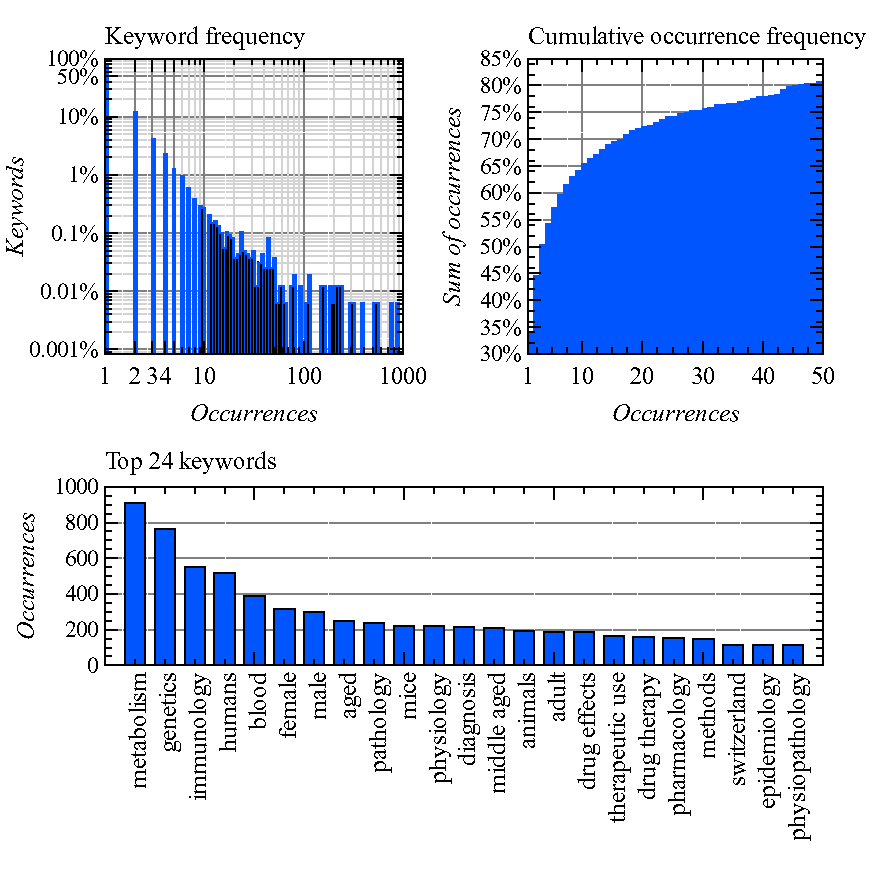
\includegraphics{images/keywords_clean_histogram_abc.pdf}
\caption{In \texttt{keywords/keywords\_clean\_histogram.json}, the
distribution of keywords is strongly skewed right (min = Q1 = M = Q3 =
1, max = 910). However, even though keywords with only one occurrence
constitute over 75\% of the total keywords, their occurrences constitute
less than 35\% of the total occurrences. The most common keywords with
50 or more occurrences are extreme outliers but make up almost 20\% of
the total occurrences.}
\end{figure}

To analyse the spread of keywords in the sample data set, the keywords
per item are counted. To do so, we call \texttt{Keywords.make\_count} on
\texttt{/indexed/indexed\_master\_mesh\_enriched.json} and save the
output as \texttt{/analysis/keywords\_counted.json}:

\begin{Shaded}
\begin{Highlighting}[]
\NormalTok{sample\_data\_set }\OperatorTok{=}\NormalTok{ Utility.load\_json(DIR }\OperatorTok{+} \StringTok{"/indexed/indexed\_master.json"}\NormalTok{)}
\NormalTok{keywords\_counted }\OperatorTok{=}\NormalTok{ Keywords.make\_count(sample\_data\_set)}
\NormalTok{Utility.save\_json(keywords\_counted, DIR }\OperatorTok{+} \StringTok{"/analysis/keywords\_counted.json"}\NormalTok{)}
\end{Highlighting}
\end{Shaded}

The median number of keywords for an item in the sample data set is 6
with an IQR of 4 (min = 0, Q1 = 4, M = 6, Q3 = 8, max = 87). Of course,
items in the sample data set with a number of keywords below the first
and above the third quartile are highly suspect from a qualitative point
of view: when it comes to subject indexing, some terms are required, but
more is usually worse {[}!! source{]}. Items with too few or too many
keywords will be discussed in more detail in section
\protect\hyperlink{assessment}{section Assessment}

\hypertarget{reconciliation}{%
\subsection{Reconciliation}\label{reconciliation}}

As explained in section X, Annif assigns index terms from a controlled
vocabulary. If we want to assess the quality of the indexing via a gold
standard, we must therefore ensure that the gold standard makes use of
the vocabulary used by Annif. As seen in section Y, the relevant
(English) vocabularies are Wikidata YSO. The next step in constructing
the derivative gold standard is hence to match the extracted and cleaned
keywords with keywords from YSO and Wikidata. This process is called
``reconciliation'' (see https://docs.openrefine.org/manual/reconciling)
and the tool of choice for this task is OpenRefine (see
\protect\hyperlink{openrefine}{section OpenRefine}).

In this section, I will describe how the cleaned keywords were
reconciled with Wikidata and YSO, and which additional steps for
refinement were undertaken. In total, 2'104 data transformation
operations were performed; the complete operation history is available
as \texttt{/keywords/operation\_history.json}.

The data from \texttt{/keywords/keywords\_clean\_histogram.json} was
imported into OpenRefine. The \texttt{keyword} column was then
duplicated and reconciled with Wikidata. Here the parameters were chosen
as follows: reconcile against no particular type, and auto-match
candidates with high confidence.

The reconciliation service API returns automatic matches (call them
``suggestions''). A suggestion is correct if and only if the meaning of
the keyword from \texttt{/keywords/keywords\_clean\_histogram.json}
corresponds to the meaning of the suggested concept from Wikidata. Note
that for homonymous or polysemous keywords, it is impossible to confirm
a correct match without further context; those keywords therefore cannot
be reconciled (but see \protect\hyperlink{construction}{section
``Construction''} for a possible solution). Unfortunately, random
sampling showed that the overall quality of the reconciliation was not
satisfactory, that is, there were too many incorrect suggestions. A
two-pronged strategy was adopted to ameliorate the quality of the
reconciliation.

First, the suggestions to the top 500 keywords were manually verified.
These keywords account for 14'996 occurrences or 40.638\% of the total
occurrences and thus constitute an effective lever.

Second, systematic biases were identified and removed. The most
prevalent bias was an due to a suggestion's type. As stated above, the
reconciliation service API was not constrained by type but had access to
the complete Wikidata database. Since Wikidata is an ontology that
encompasses everything, it also features types whose concepts cannot
qualify as subject terms (at least in the present context). The most
prominent example is the type Q13442814 ``scholarly article.'' Wikidata
contains the metadata of many scholarly articles. Now, for some of our
keywords, there is a scholarly article with a title that exactly matches
the keyword; and since there is no restriction concerning the type, the
scholarly article is suggested with high confidence (see
https://github.com/OpenRefine/OpenRefine/wiki/Reconciliation-Service-API
for details). For example, {[}keyword/article{]}. To generalize,
suggestions with types whose concepts are proper names are usually
incorrect. Based on this observation, suggestions with the following
types were rejected: ``scholarly article,'' ``clinical trial,''
``scientific journal,'' ``academic journal,'' ``open access journal,''
``thesis,'' ``doctoral thesis,'' ``natural number.'' Suggestions with
the following types were manually verified (i.e., checked for
correctness): ``human,'' ``album,'' ``film,'' ``musical group,''
``business,'' ``literary work,'' ``television series,''
``organization,'' ``family name,'' ``written work,'' ``video game,''
``single, television series episode,'' ``painting,'' ``commune of
France,'' ``city of the United States,'' ``magazine,'' ``studio album,''
``year,'' ``nonprofit organization,'' ``border town,'' ``international
organization,'' ``political party,'' ``software,'' ``song,''
``website,'' ``article comic strip,'' ``collection,'' ``commune of
Italy,'' ``fictional human,'' ``film,'' ``government agency,''
``village,'' ``academic journal article,'' ``female given name,''
``poem.''

With these improvements in place, each keyword with a suggestion was
assigned a QID via the ``Add cloumns from reconciled values''-function
(and similar for YSO and MeSH identifiers). The data was then exported
and saved as \texttt{/keywords/keywords\_reference.json}. Keywords with
a QID now constitute 69\% of all keywords and 78\% of their total
occurrences in the sample data set, but these numbers are significantly
lower for the MeSH identifier (53.6\% of all keywords with only 28.8\%
of all occurrences) and especially low for the YSO identifier (26.9\% of
all keywords with 11\% of all occurrences). In both cases, the problem
is due to the fact that Wikidata's mapping of MeSH respectively YSO is
only partial. There can be two reasons for this state of affairs for a
given entry: either there is no match between Wikidata and YSO or MeSH
(after all, Wikidata is much larger than MeSH and YSO taken together),
or there is a match but it has not yet been added to the mapping. In the
latter case, at least with respect to YSO, there is a solution: Finto
provides a REST-sytle API to access the YSO vocabulary directly (see
https://api.finto.fi/). For each keyword in the list of reference
keywords that lacks a YSO identifier, the Finto API is queried; if a
term turns up, it is added to the keyword. The effect of this second
reconcilement is detailed in Figure 4. It is achieved by calling
\texttt{Keywords.enrich\_with\_yso} on
\texttt{/keywords/keywords\_reference.json} and saving the output as
\texttt{/keywords/keywords\_reference\_master.json}

\begin{Shaded}
\begin{Highlighting}[]
\NormalTok{keywords\_reference }\OperatorTok{=}\NormalTok{ Utility.load\_json(DIR }\OperatorTok{+} \StringTok{"/keywords/keywords\_reference.json"}\NormalTok{)}
\NormalTok{keywords\_reference\_new }\OperatorTok{=}\NormalTok{ Keywords.enrich\_with\_yso(keywords\_reference)}
\NormalTok{Utility.save\_json(keywords\_histogram, DIR }\OperatorTok{+} \StringTok{"keywords/keywords\_reference\_master.json"}\NormalTok{)}
\end{Highlighting}
\end{Shaded}

\begin{figure}
\centering
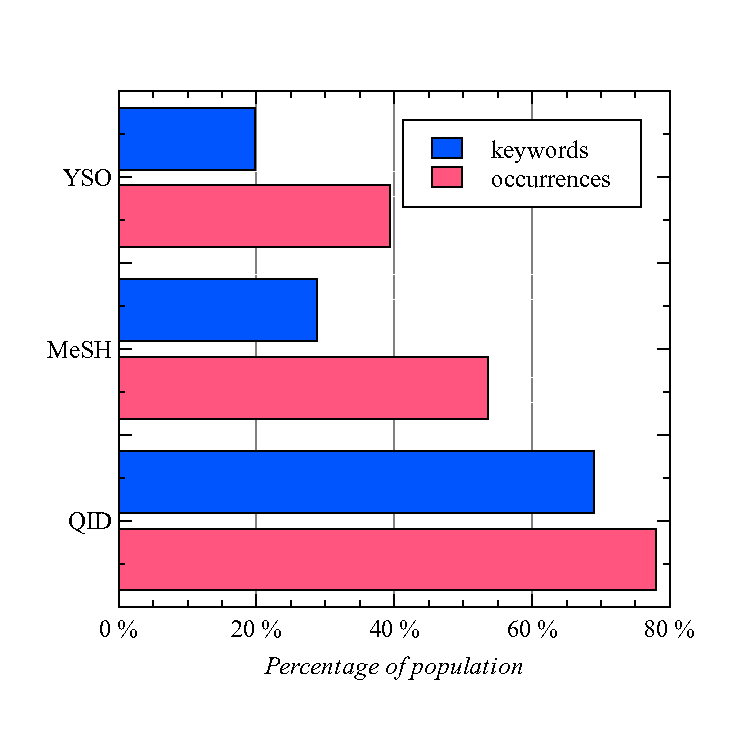
\includegraphics{images/native_gold_standard.pdf}
\caption{The coverage of
\texttt{/keywords/keywords\_reference\_master.json} by the controlled
vocabularies of Wikidata (QID), Medical Subject Headings (MeSH), and YSO
(General Finnish Ontology). Both MeSH and YSO are dependent on QID but
independent of each other. YSO enriched is the superset of YSO created
by reconciling keywords that lack a YSO identifier directly with the YSO
database provided by the Finto API; it is hence independent of
Wikidata.}
\end{figure}

Finally, consider the distribution of the cleaned and reconciled
keywords per item in the Edoc sample data set. The corresponding data is
generated with \texttt{Keywords.make\_count} as described in
\protect\hyperlink{analysis}{subsection Analysis} above and available as
\texttt{/analysis/keywords\_counted.json}. Figure 5 shows that the
median number of keywords from MeSH or YSO might be too low to be
adequate. This problem can be amended by imposing further constraints on
the sample data set and such a solution is discussed in section {[}!!
section{]}.

\begin{figure}
\centering
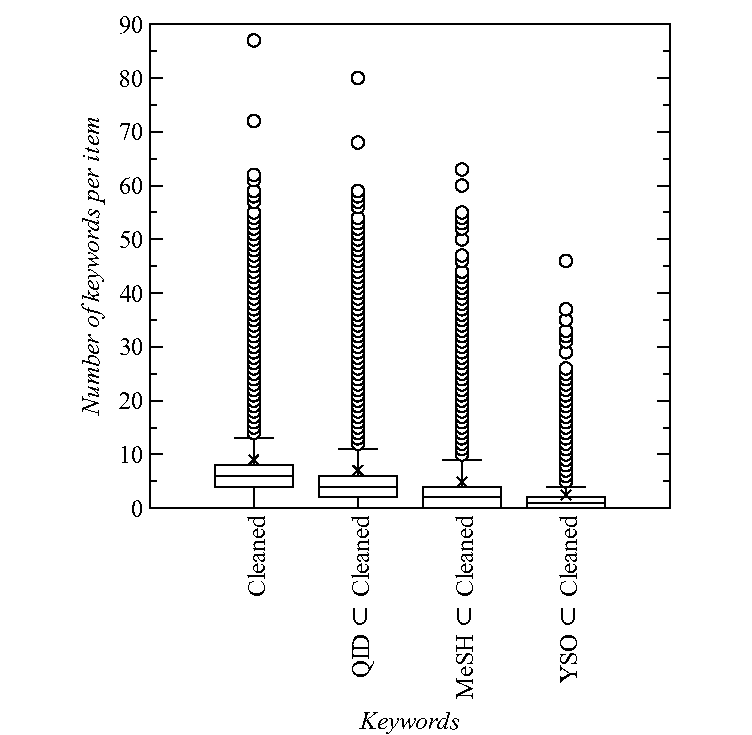
\includegraphics{images/keywords_counted.pdf}
\caption{The distribution of keywords per item in the Edoc sample data
set. The leftmost boxplot shows the distribution of cleaned keywords
(min = 0, Q1 = 4, M = 6, Q3 = 8, max = 87); the other boxplots show the
distribution of cleaned keywords with reconciled QID (min = 0, Q1 = 2, M
= 4, Q3 = 6, max = 80), MeSH ID (min = Q1 = 0, M = 2, Q3 = 4, max = 63),
and YSO ID respectively (min = Q1 = 0, M = 1, Q3 = 2, max = 46). All
four distributions are similarly consistent, but there is a linear
decrease of the distribution's center leaving MeSH and YSO with
potentially too few descriptors to represent an adequate indexing.}
\end{figure}

\hypertarget{discussion}{%
\subsection{Discussion}\label{discussion}}

Let us now turn to the evaluation of the reconciliation: how many of the
suggestions were correct? This question was answered via random sampling
(following Roth and Heidenreich 1993, 204--25). The random sample
(\(n=500\)) was created by calling
\texttt{Analysis.make\_random\_sample} on
\texttt{/keywords/reference\_keywords\_master.json}; it is available at
\texttt{/analysis/random\_keywords.json}. The sample was then imported
into OpenRefine and the judgement (1 for correct, 0 for incorrect) of
the manual verification was recorded in the column
\texttt{verification}. The data was then exported and is available at
\texttt{/analysis/random\_keywords\_verified.csv}.

An analysis of this data shows that 53\% of the suggestions in the
random sample were correct with a 95\% confidence interval of 48.8\% to
57.3\%. We can therefore conclude that 8'507 \(\pm\) 692.1 of the 16'050
keywords in \texttt{/keywords/reference\_keywords.json} have correct
suggestions. Note that of the 235 incorrect suggestions in the random
sample, 188 were incorrect by default because they were missing a QID;
the share of non-empty yet incorrect suggestions is only 9.4\% in the
random sample meaning that the quality of the reconciliation is not as
disappointing as it might seem at first glance.

\hypertarget{assessment}{%
\section{Assessment}\label{assessment}}

In this section I will assess the quality of the sample data set's
indexing with Annif based on the gold standard.

\hypertarget{precision-recall-f1-score}{%
\subsection{Precision, recall,
F1-score}\label{precision-recall-f1-score}}

The metrics used for the assessment are precision, recall and F1-score.
Precision and recall are standard metrics for indexing quality (e.g.,
Gantert 2016, 197) whereby the F1 score plays are more prominent role in
the assessment of machine indexing (e.g., Suominen 2019, 11--14; Toepfer
and Kempf 2016, 93f.). Of course, there is a host of alternative metrics
(such as indexing consistency, transparency, reproducability) that are
neglected here.

Let us briefly look at the definitions and motivations of the chosen
metrics. Remember that a suggestion of a subject term is correct if and
only if the subject term is in the derivative gold standard. The
possible outcomes are summarized in Table 1.

\begin{table}[h]
\centering
\begin{tabular}{lllll}
 &                       & \multicolumn{2}{l}{Suggested by Annif?}            &  \\ \cline{3-4}
 & \multicolumn{1}{l|}{} & \multicolumn{1}{l|}{No} & \multicolumn{1}{l|}{Yes} &  \\ \cline{2-4}
\multicolumn{1}{l|}{\multirow{2}{*}{In gold standard?}} & \multicolumn{1}{l|}{No}  & \multicolumn{1}{l|}{True negative}  & \multicolumn{1}{l|}{False positive} &  \\ \cline{2-4}
\multicolumn{1}{l|}{}                                   & \multicolumn{1}{l|}{Yes} & \multicolumn{1}{l|}{False negative} & \multicolumn{1}{l|}{True positive}  &  \\ \cline{2-4}
\end{tabular}
\caption{Annif confusion matrix.}
\label{tab:confusion-matrix}
\end{table}

``Precision'' is the fraction of the correctly suggested subject terms;
a suggestion is correct if and only if it is in the derivative gold
standard:

\begin{center} 
$\text{Precision} = \displaystyle \frac{\text{True positive}}{\text{True positive} + \text{False positive}}$
\end{center}

Or put as question: what fraction of the subject terms suggested by
Annif are also in the derivative gold standard?

``Recall'' is the fraction of correct subject terms out of all correct
subject terms:

\begin{center} 
$\text{Recall} = \displaystyle \frac{\text{True positive}}{\text{True positive} + \text{False negative}}$
\end{center}

Put as question: what fraction of the subject terms in the gold standard
were suggested by Annif?

The F1-score is the harmonic mean between precision and recall:

\begin{center} 
$\text{F1} = \displaystyle 2 * \frac{\text{Precision} * \text{Recall}}{\text{Precision} + \text{Recall}}$
\end{center}

The above scoring metrics were implemented using the scikit-learn
machine learning library (Pedregosa et al. 2011). For a given Annif
configuration
(\protect\hyperlink{annif-versus-derivative-gold-standard}{section
``Annif versus derivative gold standard''})\ldots{} {[}perhaps explain
how it is done, important to mention transformation of multilabel to
binary{]}.

\hypertarget{creating-the-data-foundation}{%
\subsection{Creating the data
foundation}\label{creating-the-data-foundation}}

I will now describe how the data foundation for the assessment was
created. There are three parameters that need to be distinguished (see
\protect\hyperlink{annif}{section ``Annif''}):

\begin{enumerate}
\def\labelenumi{\arabic{enumi}.}
\tightlist
\item
  The Annif project (algorithm plus vocabulary) responsible for the
  indexing of the sample data set. As per the Annif REST API, these are
  \texttt{yso-en}, \texttt{yso-maui-en}, \texttt{yso-bonsai-en},
  \texttt{yso-fasttext-en}, and \texttt{wikidata-en}.
\item
  The text base per item, namely title versus title and abstract.
\item
  The maximum number of suggestions per item. Since we required 10
  suggestions per item, we can choose between 1-10 suggestions.
\end{enumerate}

Combining these parameters, we really have 100 Annif configurations
whose performance we want to compare and assess: Annif project \(*\)
text base \(*\) maximum number of suggestions \(= 5 * 2 * 10 = 100\).
Each configuration has a unique ID (called ``marker'' in what follows)
constructed by the convention:
\texttt{\{project\_id\}-\{abstract\}-\{fulltext\}-\{n\}-\{threshold\}}
where \texttt{project\_id} is the Annif project, \texttt{abstract} and
\texttt{fulltext} are boolean variables, \texttt{n} is the maximum
number of suggestions per item, and \texttt{threshold} is a variable for
a threshold Annif score.

For each configuration, the F1-score was then computed. It is important
to note that each metric comes in three different flavors dubbed
``macro,'' ``micro,'' and ``weighted'' respectively (see Sokolova and
Lapalme 2009). In the macro flavor, the metric represents simply the
mean per class (i.e., correct or incorrect suggestion). The weighted
metric is the macro metric but each class is weighted by its true
positives. By contrast, a metric with the micro flavor is computed
globally over all true positives and false positives respectively
negatives. So the ``macro'' and ``weighted'' flavors are useful for
assessing the performance of a configuration with respect to individual
cases of assigning subject terms (call them ``samples'') whereas the
``micro'' flavor is most suitable to assess the overall performance of a
configuration with respect to assigning subject terms.

To compute the F1-score, we call \texttt{Analysis.super\_make\_metrics}
on \texttt{/indexed/indexed\_master\_mesh\_enriched}. The 100 output
files are saved as \texttt{/metrics/metrics\_\{marker\}.json} where
\texttt{marker} specifies the Annif configuration; a single file for
analysis is saved as \texttt{/analysis/metrics.json}:

\begin{Shaded}
\begin{Highlighting}[]
\NormalTok{Analysis.super\_make\_metrics(DIR }\OperatorTok{+} \StringTok{"/indexed/indexed\_master.json"}\NormalTok{)}
\end{Highlighting}
\end{Shaded}

Note that the data foundation includes additional information, namely
the sample size and the raw values for the confusion matrix. The sample
size is a histogram of each instance in which a value in the confusion
matrix was computed, that is, each case in which either Annif or the
derivative gold standard assigned a subject term. Finally, note that if
an item in the Edoc sample data set had an empty derivative gold
standard, no score was computed; this is the case exactly if none of the
cleaned keywords had been matched to Wikidata or YSO respectively.
Configurations with a Wikidata vocabulary had a scoring coverage of
94.38\% of the items in the sample data set as compared to only 62.84\%
for configurations with a YSO vocabulary.

\hypertarget{general-results}{%
\subsection{General results}\label{general-results}}

In this section I will discuss the general results of assessing the
performance of the 100 Annif configurations versus the derivative gold
standard with respect to the Edoc sample data set. The data foundation
is available at \texttt{/analysis/metrics.json}.

\begin{figure}
\centering
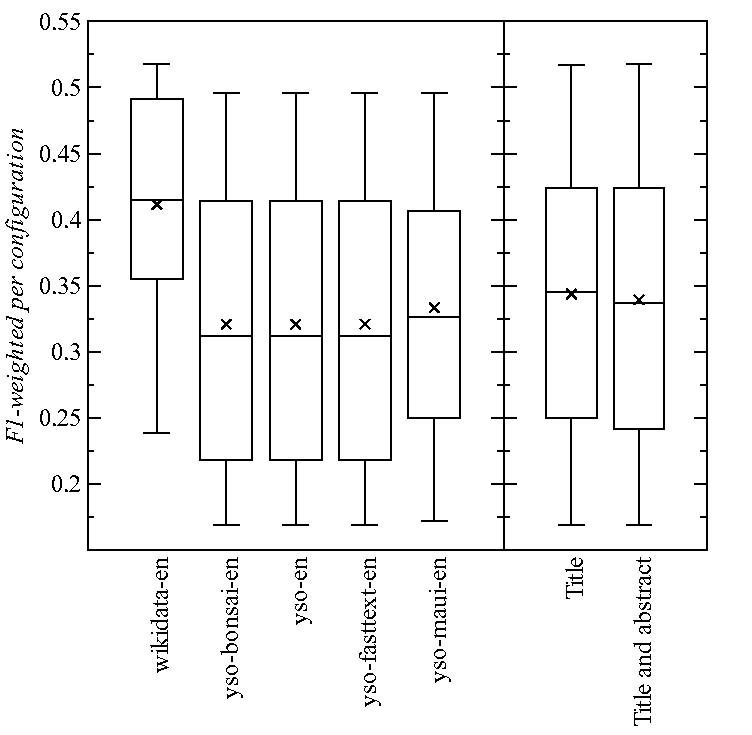
\includegraphics{images/metrics_all_project+abstract.pdf}
\caption{Distribution of weighted F1-scores per class of project of
Annif configuration (left) and per class of text basis of Annif
configuration (right). \texttt{wikidata} (min = 0.239, Q1 = 0.355, M =
0.415, Q3 = 0.492, max = 0.517) outperforms any YSO configuration.
\texttt{yso-bonsai-en}, \texttt{yso-en} and \texttt{yso-fasttext-en} are
on par (min = 0.169, Q1 = 0.218, M = 0.312, Q3 = 0.414, max = 0.496) and
slightly outperformed by the more consistent \texttt{yso-maui-en} (min =
0.171, Q1 = 0.250, M = 0.327, Q3 = 0.407, max = 0.496). Surprisingly,
the performance of configurations based on titles (min = 0.169, Q1 =
0.250, M = 0.345, Q3 = 0.424, max = 0.517) was marginally better than
the performance of configurations based on titles and abstracts (min =
0.169, Q1 = 0.242, M = 0.337, Q3 = 0.424, max = 0.517).}
\end{figure}

Let us first consider overall performance. Here the most striking result
is that Wikidata configurations outperformed YSO configurations (see
Figure 6, left). However, the explanation of this effect is not evident.
The two main explanatory hypotheses are 1. that the suggestions by the
Wikidata configurations are more salient, or 2. that the derivative gold
standard is biased towards Wikidata due to its higher coverage of QIDs
as compared to YSO IDs. By contrast, the Wikidata configurations are
more productive than the YSO configurations, and the reason for this
effect is the higher coverage of QIDs as compared to YSO IDs (see Figure
7). By ``productivity'' I mean that the absolute number of assigned
subject terms. So Wikidata configurations are not only qualitatively but
also quantitatively superior to YSO configurations.

\begin{figure}
\centering
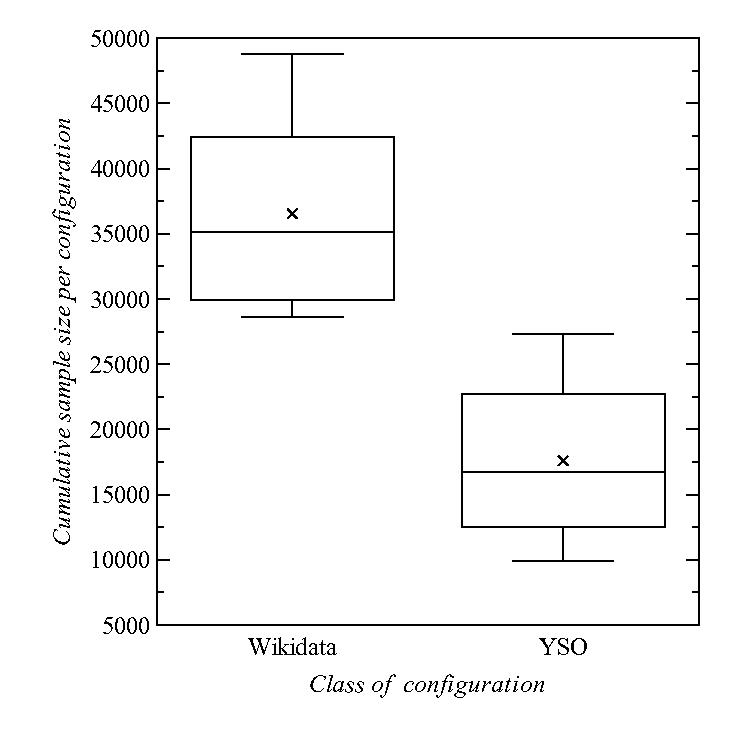
\includegraphics{images/metrics_all_productivity.pdf}
\caption{The distribution of cumulative sample size per project class of
Annif configuration. Wikidata configurations (min = 28'618, Q1 = 29'912,
M = 35'121, Q3 = 42'439, max = 48'776) are more productive than YSO
configurations (min = 9'878, Q1 = 12'546, M = 16'710, Q3 = 22'694, max =
27'354).}
\end{figure}

Furthermore, the four YSO configurations are more or less on par: the
\texttt{yso-bonsai-en}, \texttt{yso-en}, and \texttt{yso-fasttext-en}
configurations perform very similarly and are slightly outperformed by
\texttt{yso-maui-en} (see Figure 6, left). This result is consistent
with other assessments reporting that ``{[}o{]}f the individual
algorithms, Maui performed best on all corpora'' (Suominen 2019, 13).

A surprising result is that there was no performance gain achieved by
increasing the text basis from titles to titles and abstracts (see
\protect\hyperlink{creating-the-data-foundation}{section ``Creating the
data foundation''}: if anything, the performance for the extended text
basis was slightly worse (see Figure 6, right). There is again no easy
explanation for this find since there are multiple plausible causes
which cannot be distangled here. For example, the abstract of an item in
the Edoc sample data set might be less representative of the item's
content than its title. In that case, the observed worse perfomance of
the Annif configurations based on title and abstracts would even be
expected. Alternatively, it might be the case that the problem lies with
Annif: a larger text basis introduces more confounding factors and might
make it harder to extract the subject terms required. An experimentum
crucis to decide between the two discussed explanations would be to
further extend the text basis to include full texts in addition to
titles and abstracts.

\begin{figure}
\centering
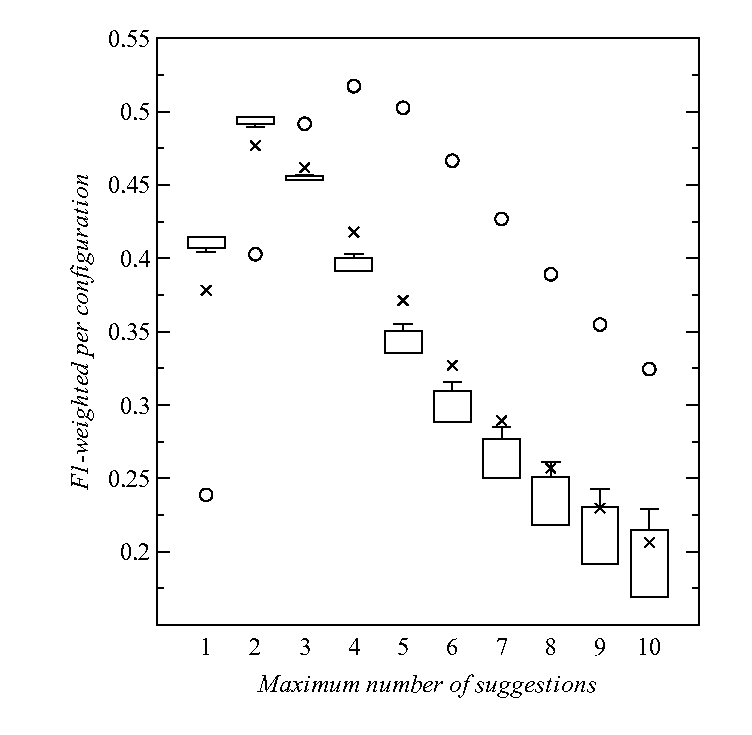
\includegraphics{images/metrics_all_n.pdf}
\caption{Distribution of weighted F1-scores per maximum number of
suggestions 1 \(\leq\) n \(\leq\) 10. See Table 2 for numeric values. n
= 2 is the best perfomring type of configuration. However, it is
outperformed by n = 4 and n = 5 token configurations. The distribution
of the distributions is skewed left. Types of configurations with a
smaller maximum number of suggestions display a more consistent
performance.}
\end{figure}

\begin{table}[]
\begin{tabular}{lllllllllll}
    & n=1   & n=2   & n=3   & n=4   & n=5   & n=6   & n=7   & n=8   & n=9   & n=10  \\ \hline
min & 0.239 & 0.403 & 0.454 & 0.391 & 0.336 & 0.289 & 0.250 & 0.218 & 0.192 & 0.169 \\
Q1  & 0.407 & 0.491 & 0.454 & 0.391 & 0.336 & 0.289 & 0.250 & 0.218 & 0.192 & 0.169 \\
M   & 0.414 & 0.496 & 0.454 & 0.391 & 0.336 & 0.289 & 0.250 & 0.218 & 0.192 & 0.169 \\
Q3  & 0.414 & 0.496 & 0.456 & 0.400 & 0.351 & 0.309 & 0.277 & 0.251 & 0.231 & 0.215 \\
max & 0.414 & 0.496 & 0.492 & 0.517 & 0.503 & 0.467 & 0.427 & 0.389 & 0.355 & 0.324
\end{tabular}
\caption{Distribution of weighted F1-scores per maximum number of suggestions 1 $\leq$ n $\leq$ 10.}
\label{tab:max-number}
\end{table}

Let us turn to the parameter of the maximum number of suggestions per
item in the Edoc sample data set (see Figure 8). Here the best
performance was achieved by a token n = 4 configuration. However, the
type n = 4 configuration performed on average significantly worse than
the type n = 3 and type n = 2 configurations. So with respect to the
maximum number of suggestions, there is a discrepancy between the best
performing token configuration and the best performing type of
configuration. This distinction is important: when choosing a
configuration for the purpose of a production system, we are usually
interested in the best token configuration. The top 20 token
configurations are summarized in Figure 9. The best performing
configuration with a weighted F1-score of 0.517 is \texttt{wikidata-en}
with a maximum number of 4 suggestions per item; the text basis (title
or abstract and title) does not matter.

\begin{figure}
\centering
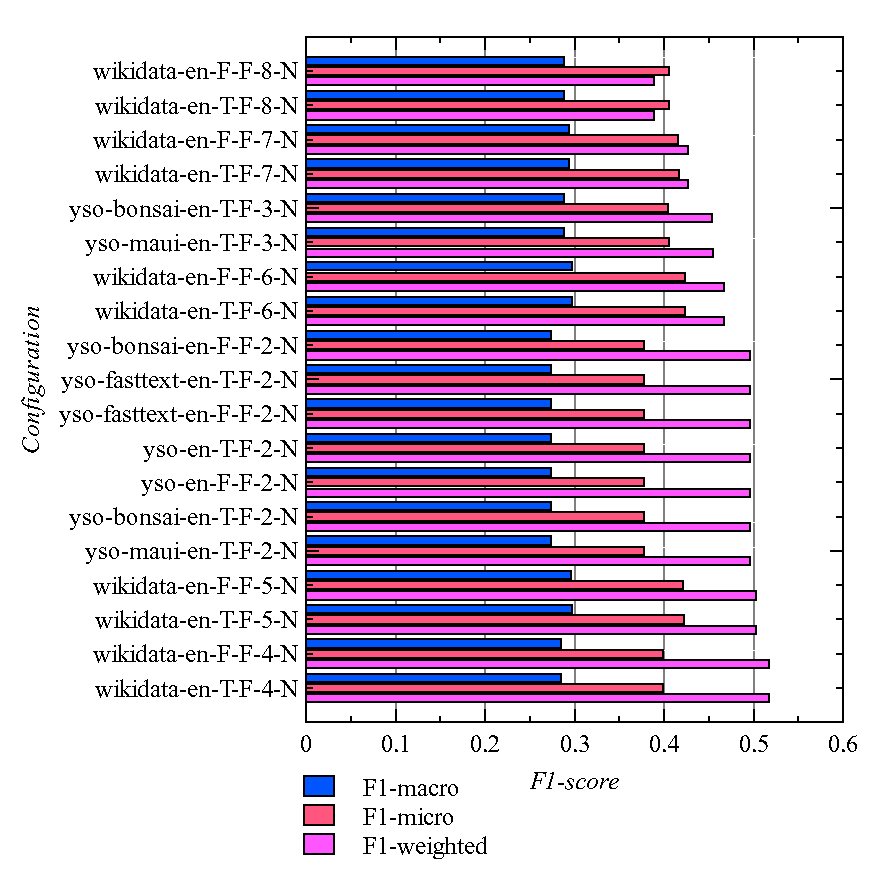
\includegraphics{images/metrics_f1_top20.pdf}
\caption{20 best performing Annif configurations (according to
F1-score).}
\end{figure}

\hypertarget{departmental-results}{%
\subsection{Departmental results}\label{departmental-results}}

In \protect\hyperlink{general-results}{section ``General results''} I
have identified and discussed the overall best Annif configerations.
However, in \protect\hyperlink{analysis}{section ``Analysis''}) I had
also noted the caveat that the performance of Annif might vary according
to department due to systematic biases in constructing the Edoc sample
data set. In this section I will therefore assess the performance of the
various Annif configurations per department.

We begin again by constructing the data foundation. Since the Edoc
\texttt{department} data field is mandatory, the sample data set is
partitioned into blocks of departments by default. We can thus create a
data foundation for each such block by calling
\texttt{Analysis.super\_make\_metrics} with a departmental parameter:

\begin{Shaded}
\begin{Highlighting}[]
\ControlFlowTok{for}\NormalTok{ dept }\KeywordTok{in}\NormalTok{ Data.get\_departments():}
\NormalTok{    Analysis.super\_make\_metrics(DIR }\OperatorTok{+} \StringTok{"/indexed/indexed\_master.json"}\NormalTok{, dept)}
\end{Highlighting}
\end{Shaded}

This yields 1000 files in
\texttt{/metrics/metrics\_\{department\}\_\{marker\}.json} (100
configurations \(*\) 10 departments) where \texttt{department} specifies
the department according to the Edoc convention. The data foundation is
summarized in \texttt{/analysis/metrics.json}.

\begin{figure}
\centering
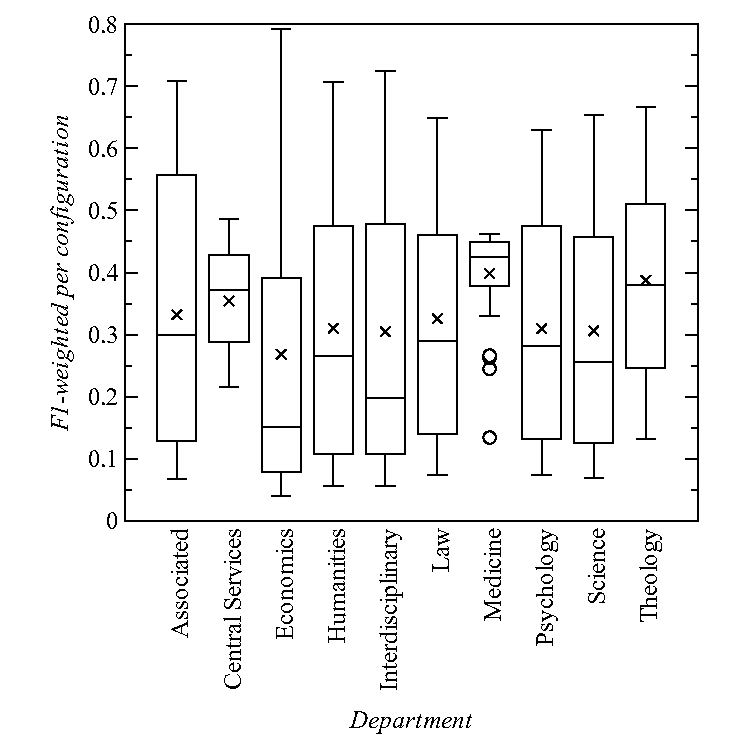
\includegraphics{images/metrics_dept_distribution.pdf}
\caption{Distribution of weighted F1-scores for all Annif configurations
per department.}
\end{figure}

Let us now look at the results. First consider the distribution of the
performance scores across departments as shown in Figure 11. We can see
that there are striking differences in variability between departments.
The departments with the most consistent weighted F1-scores are Medicine
and Central Services. However, these two departments have also the
lowest maximum weighted F1-scores. It is noteworthy that all other
departments have maximum weighted F1-scores that are well above the
F1-score of 0.517 of the best performing general Annif configuration.

\begin{figure}
\centering
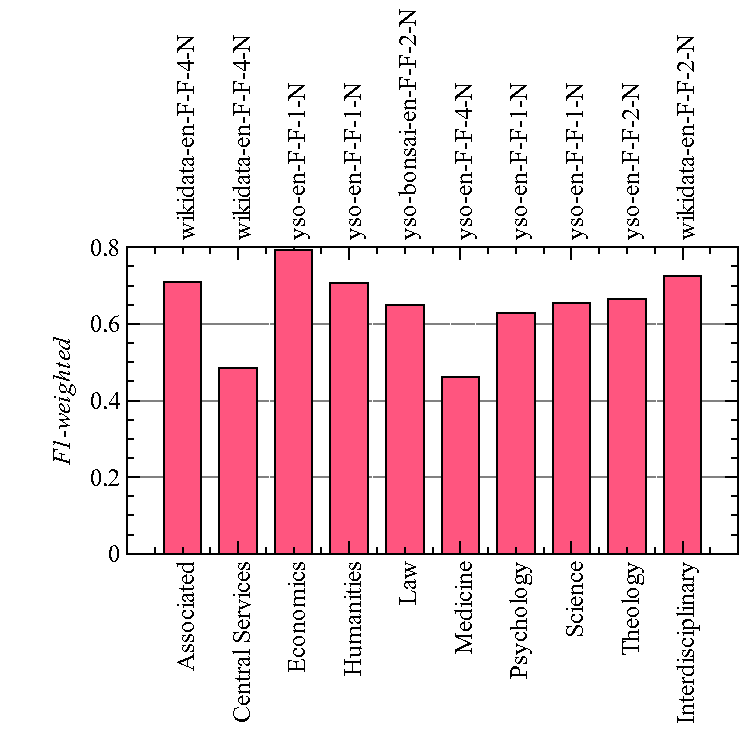
\includegraphics{images/metrics_dept_summary.pdf}
\caption{Best performing Annif configuration (according to weighted
F1-score) per department as compared to the overall best performing
Annif configuration \texttt{wikidata-en-F-F-4-N}.}
\end{figure}

Let us now consider the best performing Annif configurations per
department as summarized in Figure 12. It is evident that only two of
the ten departments (namely Associated and Central Services) have as
best performing configuration the configuration that was declared the
overall best performing configuration (namely
\texttt{wikidata-en-F-F-4-N}). More surprisingly, YSO outperforms
Wikidata in all other departments except Interdisciplinary. However, the
margin is rather slim. The notable exception is the department
Economics, where the YSO configuration outperforms the Wikidata
configuration by a factor of 3. More importantly, the best performing
YSO configurations are significantly less productive than the slightly
worse performing Wikidata configuration, except for
\texttt{yso-en-F-F-4-N} in the Medicine department.

\hypertarget{outlook-and-conclusion}{%
\section{Outlook and conclusion}\label{outlook-and-conclusion}}

\hypertarget{refinement}{%
\subsection{Refinement}\label{refinement}}

\begin{itemize}
\tightlist
\item
  fulltext support
\item
  mesh; A gold standard is usually the product of manual indexing by
  ``information experts, subject experts, or potential or real end
  users'' (Golub et al. 2016, 10). This entails its own host of
  epistemic problems relating to objectivity and consistency of the
  assigned subject terms. Most importantly, however, the construction of
  a gold standard from scratch is very expensive. It is therefore not an
  option for the project at hand. Rather, I will construct what could be
  called derivative gold standards by reusing indexing data that is
  already available. Here we can distinguish two distinct kinds of
  derivative gold standards: first, I will construct a derivative gold
  standard based on the author keywords available in the sample data
  set; call this the ``derivative'' gold standard. Second, I will
  construct a derivative gold standard based on indexing metadata
  available in repositories distinct from Edoc; call this the
  ``foreign'' gold standard. -We enrich the sample items with MeSH
  keywords from PubMed if available (item needs a PubMed ID and items
  needs to be indexed with MeSH on PubMed, 1653 items match this
  requirement); the resulting file is indexed\_master\_mesh.json. Like
  so: Data.enrich\_with\_mesh(DIR + ``/indexed/indexed\_master.json,''
  DIR + ``/indexed/indexed\_master\_mesh'')
\end{itemize}

\hypertarget{implementation-strategy}{%
\subsection{Implementation strategy}\label{implementation-strategy}}

\hypertarget{appendix}{%
\section{Appendix}\label{appendix}}

\hypertarget{bibliography}{%
\section{Bibliography}\label{bibliography}}

\hypertarget{refs}{}
\begin{CSLReferences}{1}{0}
\leavevmode\hypertarget{ref-Gantert.2016}{}%
Gantert, Klaus. 2016. \emph{Bibliothekarisches Grundwissen}. 9.,
vollst{ä}ndig neu bearbeitete und erweiterte Auflage. Berlin: {De
Gruyter Saur}. \url{https://doi.org/10.1515/9783110321500}.

\leavevmode\hypertarget{ref-Golub.2016}{}%
Golub, Koraljka, Dagobert Soergel, George Buchanan, Douglas Tudhope,
Marianne Lykke, and Debra Hiom. 2016. {``A Framework for Evaluating
Automatic Indexing or Classification in the Context of Retrieval.''}
\emph{Journal of the Association for Information Science and Technology}
67 (1): 3--16. \url{https://doi.org/10.1002/asi.23600}.

\leavevmode\hypertarget{ref-Louis.2013}{}%
Louis, Annie, and Ani Nenkova. 2013. {``Automatically Assessing Machine
Summary Content Without a Gold Standard.''} \emph{Computational
Linguistics} 39 (2): 267--300.
\url{https://doi.org/10.1162/COLI\%7B/textunderscore\%20\%7Da\%7B/textunderscore\%20\%7D00123}.

\leavevmode\hypertarget{ref-Parke.2013}{}%
Parke, Carol. 2013. \emph{Essential First Steps to Data Analysis:
Scenario-Based Examples Using SPSS}. Thousand Oaks: {SAGE Publications}.
\url{https://doi.org/10.4135/9781506335148}.

\leavevmode\hypertarget{ref-Pedregosa.2011}{}%
Pedregosa, F., G. Varoquaux, A. Gramfort, V. Michel, B. Thirion, O.
Grisel, M. Blondel, et al. 2011. {``Scikit-Learn: Machine Learning in
Python.''} \emph{Journal of Machine Learning Research}, no. 12:
2825--30.
\url{https://www.jmlr.org/papers/volume12/pedregosa11a/pedregosa11a.pdf}.

\leavevmode\hypertarget{ref-Roth.1993}{}%
Roth, Erwin, and Klaus Heidenreich. 1993. \emph{Sozialwissenschaftliche
Methoden: Lehr- Und Handbuch f{ü}r Forschung Und Praxis}. 3., v{ö}llig
{ü}berarbeitete und erweiterte Auflage. M{ü}nchen: {R. Oldenbourg
Verlag}.

\leavevmode\hypertarget{ref-Sokolova.2009}{}%
Sokolova, Marina, and Guy Lapalme. 2009. {``A Systematic Analysis of
Performance Measures for Classification Tasks.''} \emph{Information
Processing {\&} Management} 45 (4): 427--37.
\url{https://doi.org/10.1016/j.ipm.2009.03.002}.

\leavevmode\hypertarget{ref-Stokhof.2011}{}%
Stokhof, Martin, and Michiel van Lambalgen. 2011. {``Abstractions and
Idealisations: The Construction of Modern Linguistics.''}
\emph{Theoretical Linguistics} 37 (1-2): 1--26.
\url{https://doi.org/10.1515/thli.2011.001}.

\leavevmode\hypertarget{ref-Suominen.2019}{}%
Suominen, Osma. 2019. {``Annif: DIY Automated Subject Indexing Using
Multiple Algorithms.''} \emph{LIBER Quarterly} 29 (1): 1--25.
\url{https://doi.org/10.18352/lq.10285}.

\leavevmode\hypertarget{ref-Toepfer.2016}{}%
Toepfer, Martin, and Andreas Oskar Kempf. 2016. {``Automatische
Indexierung Auf Basis von Titeln Und Autoren-Keywords -- Ein
Werkstattbericht.''} \emph{027.7 Zeitschrift f{ü}r Bibliothekskultur /
Journal for Library Culture} 4 (2): 84--97.
\url{https://0277.ch/ojs/index.php/cdrs_0277/article/view/156/354}.

\leavevmode\hypertarget{ref-UniversitatBasel.2021}{}%
Universität Basel. n.d. {``Research Database of the University of Basel
User Manual.''} Edited by Universität Basel.

\end{CSLReferences}
